% File: tex/03_introduction_old.tex
% Author: Timo L. R. Halbesma <timo.halbesma@student.uva.nl>
% Version: 0.01 (Initial)
% Date created: Sat Oct 24, 2015 12:28 am
% Last modified: Wed Jun 15, 2016 07:29 PM
%
% Description: Masterthesis, Introduction

\documentclass[MScProj_TLRH_ClusterEnergy.tex]{subfiles}
\begin{document}
\section{Introduction}
\label{sec:introduction}


\subsection{The Cygnus~A Radio Galaxy}
The Cygnus constellation, denoted by the symbol `Cyg'
\citep{1922PA.....30..469R}, is found on the Northern hemisphere right in the
plane of the Milky Way, just below the well-studied Kepler Field. More
quantitatively, it is located at a declination of roughly $+27^\circ < \delta <
+54^\circ$ and a right ascension $19^{\rm h}17^{\rm m} < \alpha < 21^{\rm
h}45^{\rm m}$. The constellation was named `The Swan' by ancient Greek
astronomers and is featured as early as Ptolemy's list of constellations. Cygnus
is often referred to as the Northern equivalent of the Southern cross. The
constellation has stars well visible to the naked eye, such as its brightest
star at the tail of the Swan, Deneb ($\alpha$ Cyg, which is also part of the
Summer Triangle, an asterism together with Vega and Altair), and at the head the
optical double Albireo ($\beta$ Cyg and $\beta_2$ Cyg) that amateur astronomers
love because of the significantly different colours between the two stars. The
constellation hosts interesting deep-sky objects like the Veil nebula, a large
bright feature in the X-ray sky caused by a supernova explosion. Other
well-known, well-studied X-ray objects found in Cygnus are the (galactic) X-ray
binary Cyg~X-1, widely accepted as the first proof of the existence of black
holes, and the microquasar Cyg~X-3 system where a Wolf-Rayet star is in a binary
with a compact object. When observing the Swan at long wavelengths, one finds it
contains the very bright radio galaxy Cygnus~A. It is this object that we take a
particular interested in.


Seminal publications in the field of radio astronomy are bundled in
\citet{1982cra..book.....S}. In the following paragraphs we summarise work done
in the early days of radio astronomy from the initial detection of the bright
radio source Cygnus~A to discussions on what the cause of this energetic
phenomenon could be. In addition, we paraphrase parts of the individual
publications found in the proceedings of a four day workshop on Cygnus~A by
\citet{1996cyga.book.....C}, and the comprehensive review by
\citet{1996A&ARv...7....1C}. These publications and references therein provide
an overview of the study of Cygnus~A up to mid 1995, and we consider more recent
literature to complete the literature summary up to the present day.


In the early days of radio astronomy it is found that strong radio emission originates from Cygnus. Following up on Jansky's pioneering work using radio waves to observe the universe, amateur astronomer Grote Reber built himself a parabolic reflector with a diameter of 31.4 feet (\mytilde 9.6 meter) in his own backyard in 1937, payed for out of his own pocked with money he saved up by commuting rather than buying a car. Catching a few hours of sleep after dinner, Reber would stay up most of his nights\footnote{During the day Reber worked as a radio engineer and operator. He would work at night to avoid interference from automobile engines.} mapping out the sky at a (during the night) fixed declination. Reber is the first to note that there is `cosmic static' origination from Cygnus. He describes that there are minor maxima appearing in Cygnus at 160 megacycles \citep{1944ApJ...100..279R} and notes that the maxima are split in two at 480 megacycles, one of which is observed at $\alpha \approx 20$ and $\delta \approx 40^\circ$ \citep{reber1948cosmic}. Reber compares this observation with \citet{1948Natur.161..312B} and notices agreement with their 60 and 200 MHz observations obtained using the Lloyds-mirror technique over the sea.

\citet{1946Natur.158..234H} are first to suggest that the emission Reber detected in the Cygnus constellation originates from a discrete source, although for the wrong reasons. At a wavelength of five meters the authors observe fluctuations with a period of about half a minute originating from the direction of Cygnus. They conclude that the variation in intensity is most likely due to a small number of discrete sources subtending an angle less than 2$^\circ$. \citet{1948Natur.161..312B} think the source of emission is similar to what produces sunspots, and confirm the fluctuations of the source. Even though the conclusions in the article are wrong, the interesting legacy of this publication is the nomenclature for radio sources where the name of the constellation is followed by the letter `A' \citep{1982cra..book.....S}, such as Cygnus~A. Assuming the variations are intrinsic to the source (e.g. a shock wave), their maximum velocity can be the speed of light which yields a source size of a couple of million kilometers. As this is the same order of magnitude as the size of the Sun, the object was thought to be a radio star \citep{1949PPSA...62..491R}. It is, however, debated whether or not these fluctuations are indeed intrinsic to the source, originate in the interstellar medium or perhaps arise locally. These fluctuations are eventually found to be due to ionospheric irregularities \citep{1950AuSRA...3..234S, 1950Natur.165..422S, 1950Natur.165..423L}.

On the one hand the radio star hypothesis was still defended although the presumed intrinsic fluctuations are the reason the source was thought to be a star, on the other hand the question was raised whether the emission could originate from outside the Milky Way. The question could be answered after \citet{1951Natur.168..555S} obtained a more accurate position for Cygnus~A with an error of at most 0.25 arcsec. Given the accurate location, it was considered worth the cost of pointing the expensive optical 200-inch Mt Palomar telescope. \citet{1954ApJ...119..206B} observed that the radio source lies in the middle of a rich cluster of galaxies, but that no star or other conspicuous object is present in the center. It is concluded that the central galaxy of the cluster must be the source of the radio emission, thus, that the radio source must be extragalactic. In addition, the optical image shows a double nucleus, tidal distortion and gravitational pull between both nuclei. Therefore the radio source is thought to originate from two colliding galaxies. The most interesting implication of observing a galaxy with a higher radio than optical luminosity is that radio galaxies are now a new class of objects. However, the colliding galaxy hypothesis is eventually discarded, but a theory to explain the observed energy is not yet known thirty years later \citep{1982cra..book.....S}. Noteworthy is also the contribution of \citet{1951AuSRA...4..158M}. They observed the coinciding positions of the radio emission and the brightest member of the cluster of galaxies, but considered it highly unlikely that the radio emission could originate from a galaxy because it would be too far away. In addition, the measured uncertainty in determining the position of the radio emission did not make a strong case for this correlation.
% Radio position 1950.0 $19^{\rm h}57^{\rm m}45^{\rm s}.3 \pm 1^{\rm s}$, $+40^{\rm s}35^{\rm '}.0 \pm 1^{\rm '}$ (F.G. Smith Ibid. 170 1064 1952), nebula (== radio galaxy Cyg~A) 1950.0 19$^{\rm h}$57$^{\rm m}$44$^{\rm s}$.49, $+40^{\rm s}35^{\rm '}46^{\rm ''}.3.$

The angular size and the structure of Cygnus~A is studied at different locations with a variety of techniques. Using intensity interferometry, \citet{1952Natur.170.1061H} find that the angular size is a thousand times larger than that of stars, and that there is an asymmetry in the angular size. Obtaining data with long baseline interferometry, \citet{1952Natur.170.1063M} obtain an accurate east-west measurement and conclude that since the angular size of the galaxy and the radio source are comparable their connection established by having the same location is verified. Moreover, \citet{1952Natur.170.1065S} use a Michelson phase-switched interferometer to obtain ratios of the Fourier terms, the ratio of fringe amplitudes at two different baselines. Finally, it is found that Cygnus~A consists of two components that are well separated and appear of equal intensity instead of observing one elongated source \citep{1953Natur.172..996J}. Moreover, it is concluded that the double radio source does not coincide with the double nucleus found in the center of the optical observations by \citet{1954ApJ...119..206B}.

\newpage
buh
\newpage
beh
\newpage
bah
\newpage

--------------------------------------------------------------------------------
General information about Cygnus~A seems perfect for the introduction: \\
\url{http://chandra.harvard.edu/chronicle/0101/cyga1.html} \\
\url{http://chandra.harvard.edu/chronicle/0101/cyga2.html} \\
\url{http://chandra.harvard.edu/chronicle/0101/cyga3.html} \\
\url{http://chandra.harvard.edu/press/00_releases/press_110600cyg.html}

Begin of what Chandra website says about Cyg~A.

TODO: spectrum, redshift shows galaxy is 1 billion light years away, colliding galaxies not enough energy, synchrotron radiation is emission process (Burbidge 1958 meeting Paris?), shape cosmic dumbbell: two lobes of high energy particles half a million lightyears apart

TODO: huge power --> radio galaxies must be far away. Assuming intrinsic size is the same forall galaxies, as evidence for steady state universe versus big bang universe. Steady State --> steady decrease in angular size as function of distance to galaxies; Big Bang --> decrease in size up to certain point, then increase due to curvature of space. Much work done on measuring apparent size.

TODO: spectrum --> hot gas. Puzzling, very weird difficult to detect lines (did not expect high redshifts). Although difficulties to obtain optical data, only 3C48.

TODO: measuring redshifts. 3C48, 3C295? Schmidt 1963. Couple of papers in Nature March 16: Quasi-Stellar Objects (QSOs / quasar). Does Cygnus~A host a quasar? \citep{1963Natur.197.1037H, 1963Natur.197.1040S, 1963Natur.197.1040O, 1963Natur.197.1041G}

TODO: term Black Hole coined in 1967. What powers quasars (--> gravity). Salpeter \& Seldovich 1964: accreting black hole --> X-rays. Black hole in binary best chance of detection, this was found in Cyg~X-1 1971.

TODO: Lynden-Bell, Rees, Blandford --> magnetic field jets

TODO: origin of gas might be a galaxy merger (or cluster of galaxies merger?)

End of what the Chandra website says about Cyg~A.
--------------------------------------------------------------------------------


TODO: figure out what are the relevant parts of the book `Cygnus~A - Study of a Radio Galaxy' \citep{1996cyga.book.....C} to read. A preview of the book can be found at \url{https://books.google.nl/books?id=1t2G76HIkI8C&printsec=frontcover&hl=nl&source=gbs_ge_summary_r&cad=0#v=onepage&q&f=false}, but the individual articles can be obtained from ADS.

\\

TODO: Read the review article on Cygnus~A \citep{1996A&ARv...7....1C} and summarise the most important parts.

One finds Cyg~A at a right ascension $\alpha = 19^{\rm h} 59^{\rm m} 28.3^{\rm s}$, a declination $\delta = +40^\circ 44^{'} 02^{\rm ''}$ (J2000), and a redshift $z = 0.056075$. The coordinates and redshift are obtained from the NASA/IPAC Extragalactic Database for objects observed by \citet{1997ApJ...488L..15O}. Given its high radio output power, it is remarkable that the redshift is so low. Cygnus~A is by far the brightest nearby radio galaxy as can be clearly seen in Figure~\ref{fig:3C405RadioPowerRedshiftOutlier} adopted from \citet{1996cyga.book....1S}. Here we see the radio power as a function of redshift. The data are from the revised third Cambridge catalog for radio sources (3CR), but the quasars have been excluded. In this catalog Cyg~A is `3C~405'. It is noteworthy that 3C~405 is an outlier compared to other galaxies at similar redshift. In fact, the only galaxy with a higher radio output (for $z<1$) is 3C~280 at $z = 0.998$. As compared to this particular galaxy, it is interesting that Cygnus~A appears to emit no light in optical from its nucleus while the brightest part of 3C~280 in optical is the central region \citep{1996cyga.book....1S}.

The estimated mass is REPLACE. ``Imaging from \satellite{Einstein} showed that Cygnus~A resides within 10$^{14}$ M\Sun of hot gas nearly 1 $h_{75}^{-1}$ Mpc in extent \citep{1984MNRAS.211..981A}.''

``The gas distribution was first imaged well by the \satellite{Einstein} X-ray satellite \citep{1984MNRAS.211..981A} The best high-resolution (\satellite{ROSAT} HRI) image was made by \citep{1994MNRAS.270..173C}, and it shows a complex interaction between the radio jets and lobes of Cyg~A and the X-ray–emitting gas in the region immediately surrounding the galaxy. The overall X-ray structure has been interpreted as a cluster-scale cooling flow, as is usually found in very rich clusters of galaxies.''

``Using \satellite{ASCA}, Markevitch et al. (1999) mapped the gas temperature across the cluster and showed the existence of a hot region between Cygnus~A and the secondary X-ray peak to the northwest (in the direction of the dynamical centroid). The temperature structure could be explained by a fairly simple model involving the merger of two subclusters of similar mass colliding head-on and developing a shock between them.''


\begin{figure}[h!]
\centering
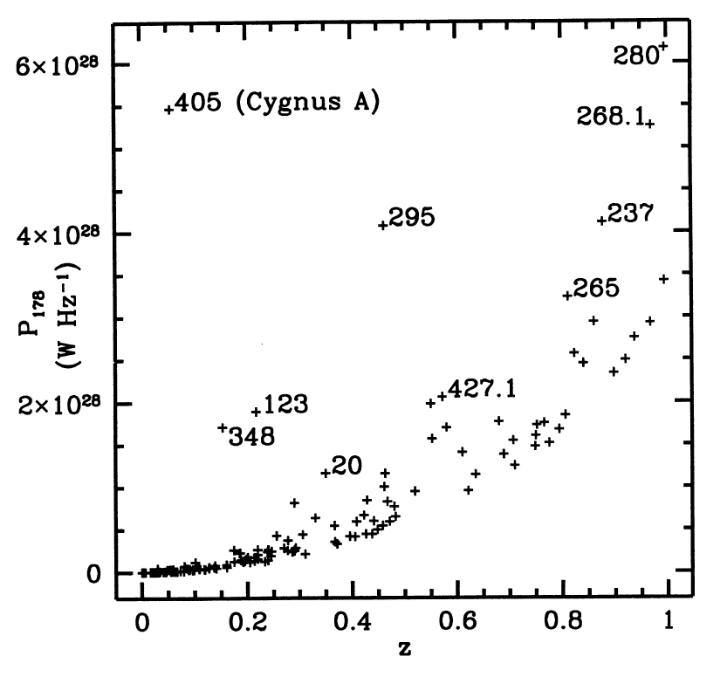
\includegraphics[width=\textwidth]{RadioPowerRedshift3C405IsOutlier.png}
\caption{Radio sources at 178 MHz (apart from quasars) in the revised third Cambridge catalog (3CR) with a redshift below $z=1$. Note that the radio power of 3C~405 (Cyg~A) is significantly higher than galaxies at similar (low) redshift. Figure adopted from \citet{1996cyga.book....1S}.}
\label{fig:3C405RadioPowerRedshiftOutlier}
\end{figure}




%, \satellite{Einstein} imaging => 10\Sup{14} M\Sun hot gas environment, 1 Mpc ($H_0 = 50$ km \Sup{-1}).

\begin{figure}[ht]
\centering
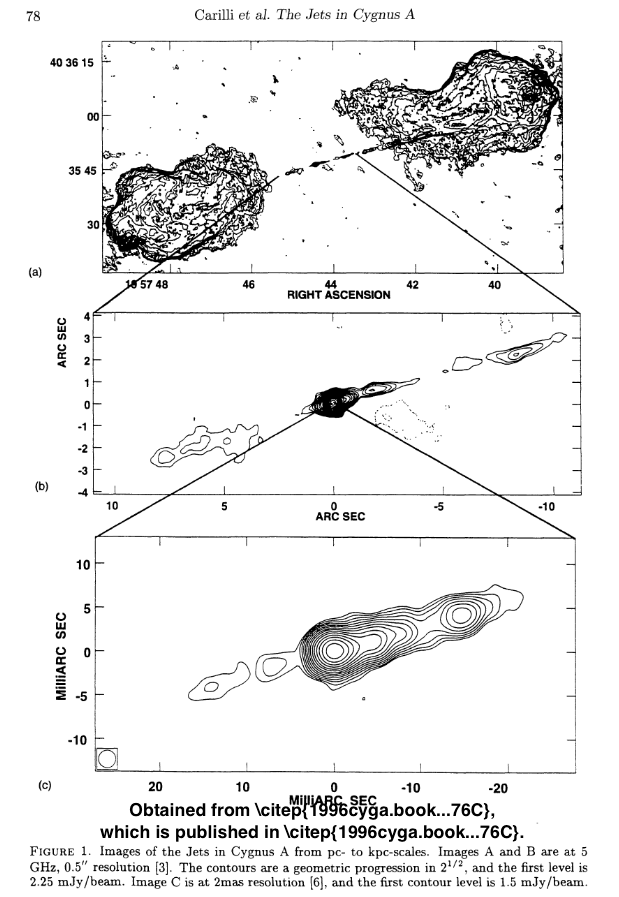
\includegraphics[width=\textwidth]{JetsInCygnusA.png}
\caption{Obtained from \citep{1996cyga.book...76C}, which is published in \citep{1996cyga.book...76C}. But it looks very similar to \citep{1996A&ARv...7....1C}, which say the image was adopted from \citep{1996cyga.book...86S}... }
\label{fig:CygAJets}
\end{figure}

\begin{figure}[ht]
\centering
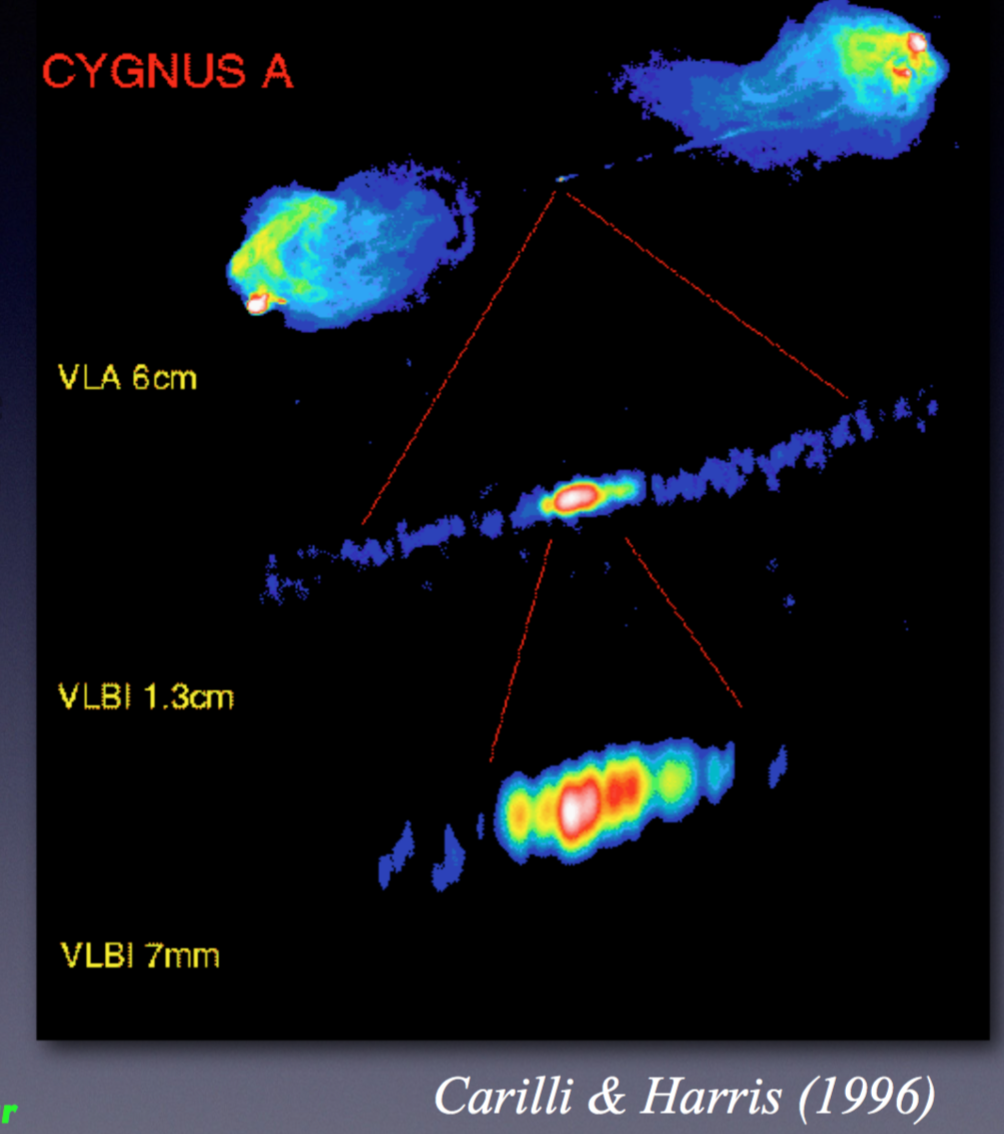
\includegraphics[width=\textwidth]{CygnusAJets.png}
\caption{Adopted from Radio Astronomy lecture slides. TODO: find the colour image instead of the black and white contour graph found in Carilli \& Harris (1996), who seem to refer to \citep{1996cyga.book...86S}.}
\label{fig:CygAJetsColour}
\end{figure}

\begin{figure}[ht]
\centering
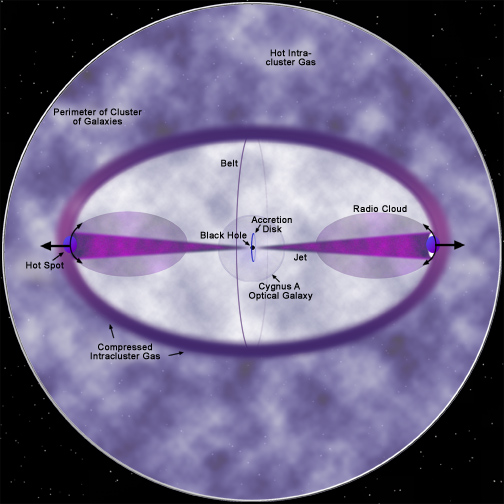
\includegraphics[width=\textwidth]{cyg_illustration.jpg}
\caption{Stolen from \url{http://chandra.harvard.edu/photo/2000/0216/cyg_illustration.jpg}.TODO: find a proper reference for this image. Image credit: NASA/CXC/K. Kowal.}
\label{fig:CygAJetsColour}
\end{figure}



\\

All references on Cygnus~A: \url{http://simbad.u-strasbg.fr/simbad/sim-id-refs?submit=sort+references&Ident=%402952489&Name=NAME+CYGNUS+A}


TODO: write something about why the Cygnus~A galaxy is epic, e.g.\ AGN, jets, heating intra cluster medium, feedback, cooling flows, .. \\

TODO: ``Cygnus~A contains a compact radio source and is the brightest of a cluster of galaxies'' \citep{1954ApJ...119..206B}
``This galaxy also contains a compact radio source and is the brightest member of a cluster of galaxies (Baade \& Minkowski 1954)" \citep{1979ApJ...230L..67F}.

TODO: calculate or obtain energy of AGN jets \\

\subsection{The Cygnus~A Cluster}
\cite{1972ApJ...178..281G} provided the second \satellite{Uhuru} satellite observational catalog which contains the X-ray source `2U~1957+40' with associated radio counterpart Cygnus~A. \citet{1974MNRAS.168..479L} did follow-up research using the \satellite{Copernicus} satellite with the aim to, firstly, verify this connection of this source with the radio galaxy Cygnus~A and to measure the spectrum, and, secondly, to study the structure of the source in X-ray. The latter goal failed due to technical problems, but the former is reached. The connection is verified and the spectrum is analysed and found in agreement with a power law of index $s = 1.3 \pm 0.6$, or with an optically thin thermal Bremsstrahlung model with $T \geq 6 \times 10^7$ K. It is argued that the simplest explanation is the thermal Bremsstrahlung model where hot cluster gas with $n_e \geq 3 \times 10^{-3}$ cm$^{-3}$ is the cause of the X-ray emission. However, they are are unable to rule out other radiation mechanisms as well as to conclude where the radiation originates from. Five years later \citet{1979ApJ...230L..67F} did succeed in studying the structure of the source using the \satellite{HEAO1} satellite. The emission appears to be extended with a size of \mytilde 2'. Furthermore it is suggested that interaction of the radio galaxy with the cluster could produce X-ray flux but that constant refueling would be required. This is similar to mechanisms suggested for the Perseus \citep{1978ApJ...224..718G} and Virgo cluster \citep{1978ApJ...219..413M}. A mass formula is adopted from the latter reference and a mass of $10^{14}$ M\Sun is inferred. The authors are aware of the complex morphology but justify the simplified assumption of an isothermal sphere to calculate a temperature ($kT$) of 6.5 keV. In addition, the following quantities are derived: a central density $n_0 \approx 0.014$ cm${^-3}$, a core radius of 0.19 Mpc, and a luminosity L$_{\rm x} \approx 5 \times 10^{44}$ erg s$^{-1}$.

A connection between the radio galaxy and the extended X-ray emission is later confirmed by \citet{1984MNRAS.211..981A}, who also focus on obtaining evidence for cooling flows. The gas is found to exhibit properties that may be caused by cooling flows, and an accretion rate of 90 M\Sun yr$^{-1}$ is inferred. Furthermore, a density profile proportional to the inverse of the radius is found. Reynolds \&



TODO: Cygnus~A, cluster of galaxies \\

TODO: paraphrase things about discovery: ``Cygnus~A was first detected as an X-ray source by Giacconi et al. (1972) using the \satellite{Uhuru} satellite (see also Longair and Willmore 1974). Follow-up observations with the \satellite{HEAO1} satellite by Fabianno et al. (1979) found that the source is spatially extended. They suggested that the emission is due to an atmosphere of hot gas with a temperature of $7 \times 10^7$ K, such as had been seen for the Virgo and Perseus clusters (see also Brinkman et al. 1977). This interpretation of a hot cluster halo for Cygnus~A was confirmed by Arnaud et al. (1984) using the \satellite{Einstein} observatory. Their IPC image shows a very extended cluster gas distribution, with a radius $\geq$ 500 h$^{−1}$ kpc, a density distribution $\propto$ radius$^{−1}$, and a total mass of $10^{14}$ M\Sun, while the \satellite{Einstein} HRI image revealed a dense core of emission, within which the radio source is embedded. The most recent treatment of the Cygnus~A cluster gas emission is by Reynolds and Fabian (1996). Using ROSAT PSPC and HRI data, they show that the cooling time for the gas within ≈ 90 h$^{−1}$ kpc is less than the Hubble time. They calculate a `cooling flow' rate of ≈ 250 M\Sun yr${−1}$ for the dense cluster gas.'' - from  \citep{1996A&ARv...7....1C}

TODO: paraphrase: ``The origin and evolution of hot cluster atmospheres is reviewed in detail in Sarazin (1986, 1988), and we refer the reader to these reviews for further details on this subject. We simply point out a few of the curiosities of the Cygnus~A cluster. First is the anisotropic distribution of the cluster gas on large-scales. The cluster shows a long ‘tail’ extending about 500 h−1 kpc to the northwest. Such a morphology implies that the system has not reached final dynamical equilibrium, perhaps indicating a recent cluster merger (time-scale ≤ cluster sound crossing time ≈ 500 Myr). And second is that optical imaging of Cygnus~A suggests that the Cygnus~A cluster is poor in galaxies, with only four galaxies identified other than Cygnus~A itself (Spinrad and Stauffer 1982). This contrasts sharply with the rich gaseous environment of the Cygnus~A cluster, and leads to questions concerning the origin and heating of the cluster gas. However, the Cygnus~A optical field is very confused, and images with sub-arcsecond resolution are required for proper determination of the true galaxy content of the Cygnus~A cluster.'' - from  \citep{1996A&ARv...7....1C}

"bla have told us one more remarkable fact about hte cluster gas and this is that it appears to be strongly magnetized ($B \mytilde 10 \mu$G)" - \citep{1996cyga.book..264B}.

TODO: merger of subclusters \\

TODO: image (Markevitch, Sarazin \& Vikhlinin 1999)  \\

TODO: Suzaku spectra: bump in Counts/s/keV vs energy keV. T (keV) vs distance along merger axis. Both in Sarazin, Finoguenov \& Wik 2012. Only 44 ksec Cycle 3 Suzaku. \\

TODO: Deep Chandra Michael --> Msec exposure. Suzaku has excellent CCD spectral resolution. TODO: find out how Chandra resolution compares to Suzaku. \\

\subsection{Merging Cygnus~A Subclusters}
``For the southwestern half of the X-ray emission in Figure 2, however, Smith et al. confirm the \satellite{ASCA} temperature results and compute both the gas mass and total integrated cluster mass. Within a 500 kpc radius, they derive a gas mass of 1.1 $\times 10^{13}$ M\Sun and a total mass between $(2.0 - 2.8) \times 10^{14}$ M\Sun (depending on the central temperature profile). We estimate a factor of 4–5 higher total mass, based on the projected mass from the optical data. However, it is hard to directly compare the two estimates, since Smith et al. assumed a lower Hubble constant (i.e., $H_0 = 50$ km s$^{-1}$ Mpc$^{-1}$) and the \satellite{Chandra} measurement includes about $\frac{1}{3}$ of the full area of the galaxy distribution and extended X-ray emission. Smith et al. (2002) also show a complex tem- perature distribution for the cluster consistent with a unsettled dynamical situation in the hot gas.'' \citep{2005AJ....130...47L}.


``Following the more classical picture of cluster cooling flows, Gomez et al. (2002) studied the consequences of head-on 4:1 and 16:1 mass-ratio mergers on existing cooling flows.'' \citep{2005AJ....130...47L}.

``The X-ray results from the literature, as discussed in \S 4.3, indicate the presence of a bow shock located between the two subclusters with a temperature enhancement a factor of 2 higher than the subcluster ICMs. A shock with these conditions is expected to form by gas moving at supersonic speeds as two approxi- mately equal mass clusters come together and reach a separation of \mytilde 1 Mpc. Such a shock forms when the leading edge of the infalling cluster is still several hundreds of kiloparsecs from the primary cluster core.'' \citep{2005AJ....130...47L}.

``The advance speed of the hotspots is supersonic and therefore we expect that the radio source is surrounded by a sheath of shocked gas (T \mytilde $1.2 \times 10^8$ K; n$_{\rm s} \mytilde 4 \times$ pre-shock, density \mytilde $4 \times 10^{-2}$ cm$^{-3}$; for the detailed numerical modelling see e.g.\ Williams \& Gull 1984)'' \citep{1984MNRAS.211..981A}

``Results from the optical one-, two-, and three-dimensional substructure analysis indicate significant bimodality, consistent with the merger of two subclusters. The level of substructure seen and the specific tests that detect it are consistent with a pre–core passage epoch, 200–600 Myr from the core crossing. Such a model is independently supported by the X-ray temperature variations and the presence of shock-heated gas between the subclusters.'' \citep{2005AJ....130...47L}.

\subsection{Connection between merger and AGN}
``In addition, the cluster-cluster merger will produce a time-variable tidal field on galaxies or dense clouds near Cygnus~A (Gnedin 2003). This could well disrupt a stable environment near Cygnus~A and cause material to fall into the core. Infalling H$_{i}$ gas is seen against the nucleus (Conway \& Blanco 1995), and recently near-IR spectroscopy has revealed a giant molecular cloud also falling into the core of Cygnus~A (Bellamy \& Tadhunter 2004). Thus, indirectly the complex cluster environment could be responsible for the extreme AGN we see in Cygnus~A.''  \citep{2005AJ....130...47L}.


\subsection{Goal of the thesis}
TODO: revise project outline written for DataNose project registration pasted below.
TODO: add scientific references to the DataNose project outline.


In the context of hierarchical structure formation it is understood why clusters of galaxies have intracluster gas at high temperatures. Cooling and heating processes influence the thermal state of this hot gas. We know cooling processes are going on because we observe cooler material, and galaxy formation implies the gas is cooling down. However, the cooling rate is lower than expected, and a significantly smaller number of big galaxies are observed than would be expected if there would not be a source of heating of the intracluster gas.

Active galactic nuclei (AGN) are possible sources that could inject sufficient energy into the ambient medium to suppress cooling of the intracluster gas. AGN are thought to be powered by super massive black holes (SMBH), a black hole with a typical mass of 10$^6$ to 10$^{10}$ times the mass of the sun located in the galactic center. As the SMBH is accreting matter from the innermost kilo parsecs of the galaxy, violent collimated outflow accelerates electrons to relativistic velocities over distances up to several kilo parsecs. These jets emit synchrotron radiation, thus, are visible at long wavelengths.

In addition, shocks arising due to merger activity are also considered to be a major contributor to heating the gas. The intracluster medium has a typical temperature of ten to hundred million Kelvin and emits thermal Bremsstrahlung, which can be observed at short wavelengths. Merger activity can be traced using this X-ray emission from the hot intracluster gas. A multi wavelength observational approach in radio and X-ray is therefore required to fully comprehend the physics in these complex systems, but in this thesis we will narrow our focus to the X-ray emission in particular.

`Cygnus~A' is an AGN, initially discovered by radio astronomy pioneer Grote Reber in 1939 and at present still one of the brightest radio sources in the sky. The Cygnus~A galaxy is the central, and therefore the biggest and brightest, galaxy of the Cygnus~A Cluster.  Interestingly, the Cygnus~A Cluster is currently undergoing a merger between two sub-clusters. The scope of this project will further be limited to this specific system. Time permitting, other systems could be analyzed too.

Specifically, we are interested in whether the cluster merger process occurring at the mega parsec scale affects the innermost kilo parsecs of the galaxy, and if so how. For instance, the cold gas reservoir surrounding Cygnus~A could be disturbed as a result of the merger, which could lead to a higher accretion rate, in turn leading to an increase in AGN activity. We will investigate whether this is the case by setting up a numerical simulation of the Cygnus~A Cluster where we trace the hot intracluster gas under the influence of gravitational and hydrodynamic equations governing the system. Initially we will represent the merger as the collision of two spherical sub-clusters with different masses. Each sub-cluster will consist of a dark matter halo and hot gaseous component. As initial conditions for the simulation, we will assume the density and temperature profiles are determined by hydrostatic equilibrium. Temperature and/or density jumps are expected characteristics of shocks, thus, of energy injection into the system. The numerically obtained temperature profile can therefore be used to probe the energy injection as a result of the cluster merger. We want to measure the amount of kinetic energy deposited into the ICM by the merger and also where that energy deposition occurs. Furthermore, the cluster merger energy will be compared to the typical AGN output energy obtained from the literature. Additionally, the simulated merger system will be compared to high resolution X-ray observations obtained from the Chandra data archive. Time-permitting, additional underlying models could be simulated and programmed into a fitting loop to study the observed data, and even other merger systems could be analyzed.

For this project it is essential to study the literature on merging galaxy clusters in general, shock physics in general, and specifically the literature on shock physics in merging galaxy clusters, as well as familiarizing myself with running hydrodynamic and gravitational simulations and, more importantly, combining both physical phenomena in the same code. Lastly, since the simulation results will be compared to new, deep Chandra observations of the Cygnus~A system, basic knowledge of `Chandra Interactive Analysis of Observations', or CIAO in beneficial for this project.

\section{Michael Chandra Proposal}
From ``The Rise to Power: Half a Billion Years of Intense AGN Activity in the Merging Cluster Cygnus A'' we obtain the following regarding the merger, including interesting references.

``Finally, on the largest scales, the sub-cluster containing Cygnus A is undergoing a nearly equal mass merger that is driving a shock into the outer cluster atmosphere and could be contributing to the high level of AGN activity observed [10, 17, 18, 19, 20, 16]'' \\

[10] Smith D. A. et al., 2002, ApJ, 565, 195 \\
[17] Owen F. N., Ledlow M. J., Morrison G. E., Hill J. M., 1997, ApJ, 488, L15 \\
[18] Markevitch M., Sarazin C. L., Vikhlinin A., 1999, ApJ, 521, 526 \\
[19] Ledlow M. J., Owen F. N., Miller N. A., 2005, AJ, 130, 47 \\
[20] Sarazin C. L., Finoguenov A., Wik D. R., 2013, Astronomische Nachrichten, 334, 346 \\
[16] Wise M. W., de Vries, M. N., Rafferty D. A., McKean J. P., 2016, in preparation \\

``Existing Chandra observations reveal a pronounced surface brightness discontinuity, roughly elliptical in shape, and surrounding the radio source in Cygnus A (see Fig. 1). This discontinuity has been interpreted as the cocoon shock inferred by Carilli, Perley \& Dreher [40] and studied previously by Wilson, Smith \& Young [13], who derived a Mach number of ~ 1.3 and a total kinetic power of ∼ $1 \times 10^46$ erg s$^−1$ . Similar values of M ~ 1.37 and ~$4 \times 10^45$ ergs$^−1$ were obtained by Nulsen [15] from fits to a spherically symmetric shock model. An analysis of the azimuthal variation in the shock yields a range of Mach values from ~1.2–1.8 [16] and may reflect asymmetries in the environment of Cygnus A due to ``cluster weather'' [41, 42] or precession of its jets [43]. Spectral mapping based on the existing 232 ksec archival Chandra data has also revealed evidence for a temperature jump in the ICM associated with the shock edge and consistent with the Mach values determined from the surface brightness [16].'' \\

[40] Carilli C. L., Perley R. A., Dreher J. H., 1988, ApJ, 334, L73 \\
[13] Wilson A. S., Smith D. A., Young A. J., 2006, ApJ, 644, L9 \\
[15] Nulsen P. E. J., 2014, in preparation \\
[16] Wise M. W., de Vries, M. N., Rafferty D. A., McKean J. P., 2016, in preparation \\
[41] Brüggen M., Ruszkowski M., Hallman E., 2005, ApJ, 630, 740 \\
[42] Morsony B. J., Heinz S., Bru ̈ggen M., Ruszkowski M., 2010, MNRAS, 407, 1277 \\
[43] Heinz S., Brüggen M., Young A., Levesque E., 2006, MNRAS, 373, L65 \\

``Unfortunately, the current data does not detect the temperature jump around the full circumference of the shock, but only at the leading edges close to the hotspots and the binning required to achieve a significant detection precludes resolving the shock temperature structure in detail. Nonetheless, these results clearly indicate that the cocoon shock in Cygnus A is depositing a significant amount of energy into the surrounding cluster gas and provides a good estimate for the mean jet power during the current outburst of Cygnus A. The requested deeper image will resolve the shock front itself on ∼ 1–2 kpc scales and at ∼ 30 positions distributed angularly around the shock boundary, especially in the region of the hotspots. It will also be possible to measure temperature jumps along small sections of the front, to verify that it is a predominantly hydrodynamic shock.'' \\

''On the scale of the merging system itself, the ICM surrounding Cygnus A shows an asymmetric morphology with an extension in the X-ray emission roughly aligned with the major axis in the radio galaxy. This asymmetry has been noted previously [10] and extends to well over ~ 200 kpc from the center of Cygnus A (see Fig. 2). Its origin is unclear, but may represent cluster gas that has been displaced and compressed by relativistic material that has passed through the hot spots at the ends of the jets. Similarly, a dramatic filamentary structure roughly ~ 280 kpc $\times$ 60 kpc is clearly seen located between the two merging sub-clusters at a radius of ~ 300 - 400 kpc and exhibits a temperature of ~ 9 keV, albeit with large uncertainties again due to the low surface brightness. This filament falls within the interstitial shock region between the two merging sub-clusters in Cygnus A and is consistent with the temperature jump associated with this region detected in lower spatial resolution data [18, 20, 16]. Mass estimates for the NW sub-cluster imply that Cygnus A is undergoing a 2:1 mass merger; however, this sub-cluster is very far off-axis in the current dataset and the effective exposure is low making the mass ratio determination uncertain. Dynamical modelling of the system favours a timeframe for the merger ∼ 0.5 Gyr prior to core passage [19].''\\

[10] Smith D. A. et al., 2002, ApJ, 565, 195 \\
[19] Ledlow M. J., Owen F. N., Miller N. A., 2005, AJ, 130, 47 \\

``Taken together, these features imply a dynamic environment surrounding Cygnus A over the past ~ 500 Myr. The proposed deeper exposure will provide accurate estimates for the energetics of these features and constrain variations in the energy output of Cygnus A on timescales ~ 300 Myr. At the same time, we will derive better constraints on the merger itself, in particular the mass ratio and associated shock, to study how this ongoing merger has affected activity in Cygnus A over the past ~ 1 Gyr.'' \\

``As the Faraday RM is proportional to the integral of the line-of-sight magnetic field weighted by the thermal electron density, an accurate 3D model of the density from X-ray observations is vital to deduce field strengths.'' -- But this is at 30 kpc, right?


\SubfileBibliography
\end{document}
